\documentclass[11pt,xcolor={dvipsnames},hyperref={pdftex,pdfpagemode=UseNone,hidelinks,pdfdisplaydoctitle=true},usepdftitle=false]{beamer}
\usepackage{presentation}
\begin{document}

\title{Presentation of ``Title of Interesting Paper'' by Author Name (Paper Year)}
\information%
{Student Name}%
{Presentation Date}
\frame{\titlepage}

\begin{frame}
\frametitle{Context: How does the paper relate to the lecture material?}
\begin{itemize}
\item This paper reviews unusual uses for olive oil throughout the Mediterranean world 
\begin{itemize}
\item It highlights in particular the challenges arising from excessive or unorthodox consumption of olive oil
\end{itemize}
\item The paper therefore contributes to our knowledge about olive oil and its consumption
\item The paper also complements the historical analysis presented in lecture
\end{itemize}	
\end{frame}

\begin{frame}
\frametitle{Question: What is the research question addressed by the paper?}
\begin{itemize}
\item The paper asks how many liters of olive oil are consumed on average per adult across 12 Mediterranean countries.
\item The paper also constructs average oil consumption over time, from 1910 to today.
\item Lorem ipsum dolor sit amet, consectetur adipiscing elit, sed do eiusmod tempor incididunt ut labore et dolore magna aliqua.
\item Ut enim ad minim veniam, quis nostrud exercitation ullamco laboris nisi ut aliquip ex ea commodo consequat.
\end{itemize}	
\end{frame}

\begin{frame}
\frametitle{Answer: What are the main elements of the answer to the research question?}
\begin{enumerate}
\item Compute the number of liters of olive oil consumed per country
\item Assess the number of adults consuming olive oil
\item Repeat for all 12 countries and all years
\item Methodological contribution: paper develops new formula to aggregate consumption:
\begin{equation*}
1+\lambda\exp{\frac{\beta}{\alpha^2}} = \max_{t}\left(x(t)-y(t)+z(t)^2 - 2\exp(\Gamma)\exp(\zeta)\exp(\kappa)\right)
\end{equation*}
\item Finds an average consumption of \al{12 liters per adult}
\begin{itemize}
\item Growing over time
\item Larger in Greece
\end{itemize}
\end{enumerate}	
\end{frame}

\begin{frame}
\frametitle{Graphical illustration of the answer to the research question}
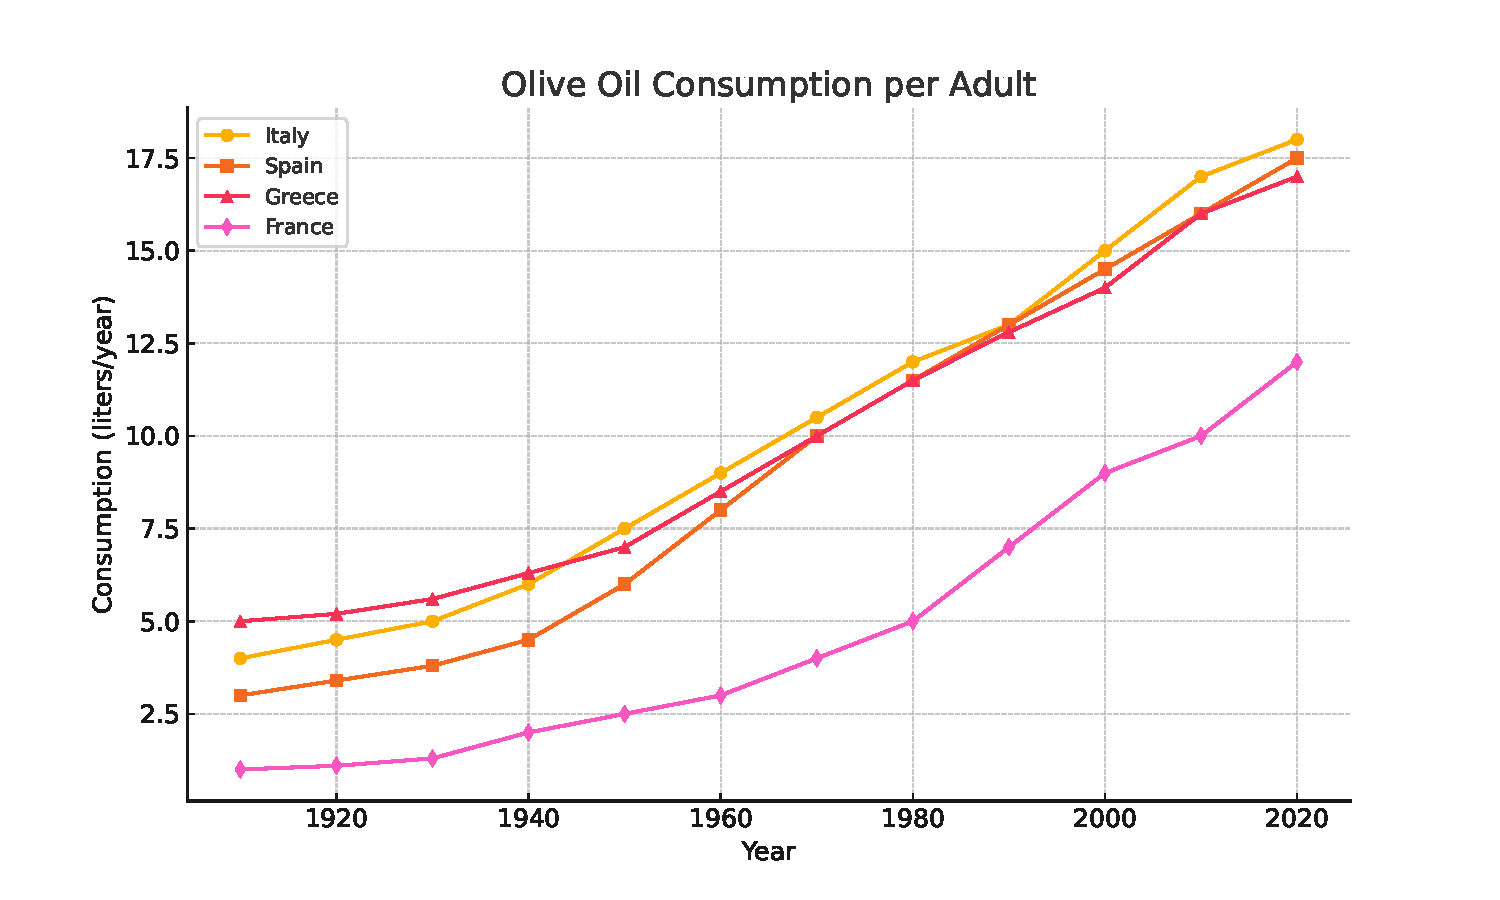
\includegraphics[scale=0.5]{olive.pdf}%
\end{frame}

\begin{frame}
\frametitle{Positioning: How does the material in the paper contribute to the previous  literature?}
\begin{itemize}
\item Previous research focused on consumption of tomatoes and cheese in the Mediterranean world
\begin{itemize}
\item Basis of Mediterranean diet (Reference 1, Reference 2)
\end{itemize}
\item But it was not known how much olive oil was consumed 
\begin{itemize}
\item Olive oil has well known medicinal properties (Reference 3)
\item[\then] But hard to assess the effectiveness of the Mediterranean diet without this information
\end{itemize}
\item The paper therefore adds information on consumption of key ingredient of well-known diet to the literature
\end{itemize}	
\end{frame}

\begin{frame}
\frametitle{Conclusion}
\begin{itemize}
\item Summarize rapidly the results
\begin{itemize}
\item Lorem ipsum dolor sit amet
\item Consectetur adipiscing elit
\item Duis aute irure dolor in reprehenderit in voluptate velit esse cillum dolore eu fugiat nulla pariatur: $\sin(\theta) = x^2 - \exp(1+\chi)$. 
\end{itemize}
\item Discuss the broader implications of the paper's results	
\item Describe the limitations of the answer provided in the paper: How could the answer be improved? 
\item What else would you have liked to know or learn on the topic?
\item Quis nostrud exercitation ullamco laboris
\end{itemize}	
\end{frame}

\end{document}